\chapter{Introduction} \label{ch:introduction}

One of the fundamental questions facing biologists is deciphering how the information in our genomes shapes our physiology and behavior.
In the past, addressing this question has been difficult due to a lack of genomic data.
However, with over 2000 genomes sequenced and the number expected to increase exponentially\footnote{\url{http://www.ncbi.nlm.nih.gov/genomes/static/gpstat.html}}, we are at the cusp of unraveling the intricacies of information contained in genomic sequences.
This flood of data has also led to creation of entirely new fields of science including that of bioinformatics and systems biology.
However, as Dobzhansky put it, ``Nothing in biology makes sense except in the light of evolution" \citep{Dobzhansky73}.
Thus, my doctoral dissertation work is primarily based on explaining genomic patterns by combining models from both molecular and evolutionary biology.
Specifically, this work integrates mechanistic models of specific biological processes such as protein translation with classical models in population genetics.

One of the earliest patterns to be discovered in genomic DNA was that of biases in codon usage \citep{Fitch76,GranthamEtAl80, Ikemura81}.
The genetic code is highly redundant with multiple codons coding for a particular amino acid (Fig. \ref{fig:genet.code}).
However, the frequency with which these codons are used within a genome are not uniform.
There exists strong preference for certain codons over others.
This preferential usage of codons is often referred to as Codon Usage Bias (CUB).
Patterns of codon usage have been found in all three domains of life: Archaea, Eubacteria and Eukaryotes \citep{CarboneEtAl03, MougelEtAl04, Subramanian08}.
Moreover, the codon usage changes not only among different organisms, but also between genes of a species as well as within a single gene.
For many organisms this preferential use of certain codons is strongly correlated with corresponding tRNA abundances and gene expression levels \citep{Ikemura81,DongEtAl96,KanayaEtAl99}.
Identifying and explaining the evolutionary forces that shape these patterns has been the focus of a large number of studies spanning over three decades.

\begin{figure}[!ht]
\begin{center}
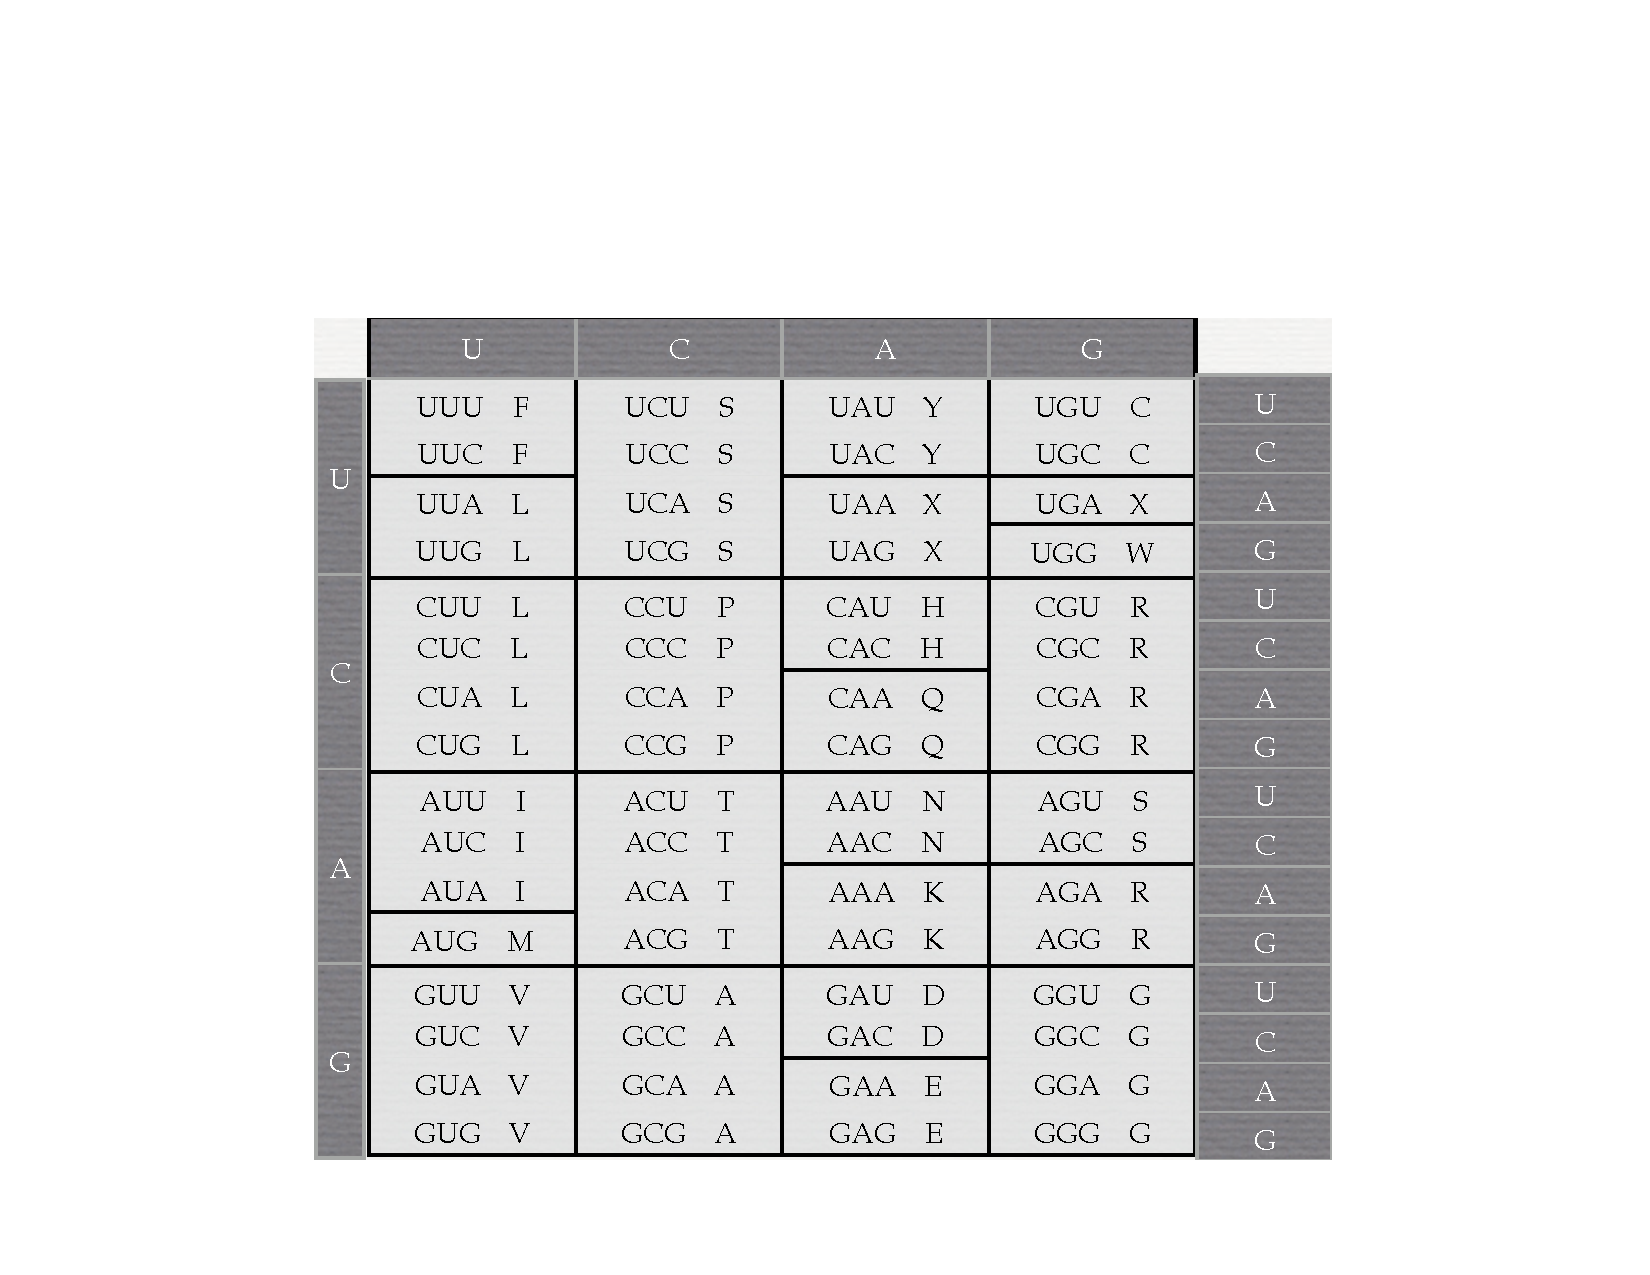
\includegraphics[width=5in]{../Figure/c1Fig_1.pdf}
\end{center}
\caption{The Genetic Code}
\label{fig:genet.code}
\end{figure}


A variety of explanations have been put forth to explain these patterns of CUB.
These explanations can be broadly classified into adaptive and non-adaptive mechanisms.
Non-adaptive mechanisms include genetic drift, and biased mutation and gene conversion.
Adaptive explanations for CUB comprise of selection for translation efficiency, selection for translation accuracy, selection against nonsense errors, selection against ribosomal interference, and selection for DNA packaging.
In multicellular eukaryotes such as humans, the effective population sizes of the species are low and the efficacy of selection in maintaining optimal codons in gene sequences is expected to be weak  \citep{ChamaryEtAl06}.
Hence, in these organisms patterns of codon usage are thought to be primarily driven by non-adaptive forces.
In contrast, in genomes of prokaryotes and unicellular eukaryotes, owing to their large effective population sizes, CUB in highly expressed genes is thought to be a result of natural selection.
However, the relative importance of various selective forces in shaping these patterns remains an area of intense debate as multiple combinations of these forces can lead to similar patterns of codon usage.
I briefly describe the various adaptive mechanisms proposed to explain CUB below.

\section{Patterns and Explanations for CUB}
\subsection{Role of translation errors}
Protein production is the most energetically expensive metabolic process within a cell \citep{Warner99, AkashiAndGojobori02}.
However, like all biological processes, protein translation is prone to errors. 
The biological importance of these translation errors and their impact on coding sequence evolution, especially the evolution of codon usage bias (CUB), depends on both their effects on protein function and their frequencies.
Translation errors fall into two categories: nonsense errors and missense errors. 

Nonsense errors have a number of different causes such as ribosome drop-off, improper translation of release factors, and frame shifts \citep{Menninger77,Kurland92,KurlandAndGallant96}. 
In addition to the indirect cost of ribosome usage, nonsense errors impose a direct assembly cost to the cell.
These costs are proportional to the length of the peptide at the time of the error \citep{Bulmer91, Kurland92, EyreWalker96,GilchristAndWagner06}.
Although costly to produce, the vast majority of these incomplete peptides are expected to have no utility for the cell \citep{KurlandAndGallant96}.

Missense errors are primarily caused by competition between cognate and near-cognate tRNAs \citep{KramerAndFarabaugh07, FluittEtAl07} followed by errors during initial tRNA selection and proof-reading \citep{RodninaAndWintermeyer01, GromadskiAndRodnina04, WintermeyerEtAl04,ZaherAndGreen09a}.
Missense errors can lead to inactive or non-functional proteins, protein aggregation, nonsense errors and in some cases even cell death \citep{CornutAndWillson91, KurlandAndGallant96, ZhaoEtAl05,  LeeEtAl06}.
However, unlike most nonsense errors which result in a non-functional protein, current data suggests that only $\sim$10-50\% of missense errors disrupt protein function \citep{MarkiewiczEtAl94,GuoEtAl04}.

Direct  estimates  of nonsense and missense error rates in prokaryotes suggest they occur with similar frequencies, i.e. on the order of  $10^{-4}$ to $10^{-3}$ per codon \citep{Manley78,TsungEtAl89,JorgensenAndKurland90,OgleAndRamakrishnan05, KramerAndFarabaugh07}).
Although these error rates may seem low, it is important to remember that these values are on a per codon basis and most coding sequences consist of hundreds of codons.
For example, a translational error rate of $10^{-3.5}$ implies that for the average length protein $\sim$1 out of every 5 proteins will contain at least one  error.

For over 30 years, the standard model of translation errors has implicitly assumed that for any given amino acid, the translation error rates are lowest for the codon with the highest tRNA abundances \citep{Ikemura81, VarenneEtAl84, KramerAndFarabaugh07}.
Surprisingly, this assumption has not been adequately tested either theoretically or empirically until now. 
In Chapter \ref{ch:trna.codon} \citep{ShahAndGilchrist10b} we directly test this assumption and find that tRNA abundances are highly correlated, i.e., tRNAs with similar abundances are clustered within the genetic code. 
This pattern is observed across a wide range of bacterial genomes. 
%In addition, we find that if tRNA abundances are positively correlated, then codons corresponding to higher tRNA abundances do not always lead to lower missense error rates.
Using a model of tRNA competition we also show that codons with higher tRNA abundances do not always lead to lower error rates. 
If correct, this represents a major shift in our understanding of how tRNA abundances affect error rates and brings into question one of the fundamental assumptions made in decades of studies on codon usage patterns.

\subsection{Role of translation efficiency}
In addition to the cost of errors during protein translation, there are major indirect costs such as the cost of ribosome production.
For example, in \emph{S. cerevisiae} during log-growth phase, $2\times10^3$ ribosome are produced every minute tying up $\sim$60\% of the cell's transcriptional machinery \citep{Warner99}.
Given their substantial cost, the efficient usage of these ribosomes during protein production is clearly advantageous and, therefore, one of the main explanations for the evolution of CUB \citep{Bulmer91}.

In Chapter \ref{ch:treff} we test the ability of a mechanistic model based on overhead cost of ribosome usage in protein production to explain and predict patterns of CUB.
This is in contrast to most commonly used indices of CUB, such as  $F_\text{\emph{op}}$ \citep{Ikemura81}, \emph{CAI} \citep{SharpAndLi86}, and \emph{CBI} \citep{BennetzenAndHall82}, which are both heuristic and aggregate measures of CUB and fail to explicitly define the factors responsible for the evolution of CUB.
I find that our model can explain $\sim$92\% of the observed variation in CUB across the \emph{S. cerevisiae} genome indicating that cost of ribosomal usage may indeed be a dominant force in shaping CUB.
Although, ours is not the first attempt at using mechanistic models to explain CUB in a population genetics context \citep{Bulmer91,Gilchrist07}, it is unique in its ability to estimate codon-specific parameters and quantitatively predict how codon frequencies change with gene expression.
In addition the framework created in this study will allow explicit comparisons of various hypothesis proposed to explain patterns of codon usage and resolution of this long-standing debate.
Moreover, the generality of our approach allows us to apply our model to any sequenced organism with available gene expression datasets.

\subsection{Role of mRNA secondary structure in affecting gene expression}
The protein production rate of a gene determines the efficacy of natural selection in affecting patterns of codon usage.
Since protein translation is limited by the rate of translation initiation \citep{Bulmer91,DeSmitAndVanDuin90}, selection for efficient usage of ribosomes would not only favor faster codons to increase the pool of free ribosomes within the cell but also affect the secondary structure of an mRNA for rapid initiation.
This is due to the fact that secondary structure of an mRNA affects the rate at which ribosome `jump' onto the mRNA.
If the mRNA structure is such that the ribosome binding site (RBS) is sequestered in a closed hairpin structure, the ribosome cannot recognize it and hence cannot initiate protein translation  \citep{YuzawaEtAl93, NakahigashiEtAl95, MoritaEtAl99,NarberhausEtAl06}.
Hence, one would expect selection for less stable secondary structures near the RBS of an mRNA.
It has been recently shown that mutations affecting the stability of mRNA secondary structures near the RBS site are correlated with changes in gene expression such that mRNAs with mutations that destabilize the structure lead to higher expression \citep{KudlaEtAl09,TullerEtAl10b}.

In Chapter \ref{ch:rna.thermo} we test the relationship between mRNA secondary structure and temperature in RNA thermometers.
RNA thermometers are genes whose expression level changes with temperature due to changes in the stability of its mRNAs  \citep{YuzawaEtAl93, NakahigashiEtAl95, MoritaEtAl99}.
At lower temperatures, the sequence adopts a secondary structure that sequesters RBS of a gene, hence interfering with translation initiation by the ribosome. 
At higher temperatures, the mRNA �melts�, increasing the accessibility of the RBS leading to an increase in the initiation of translation and, in turn, its protein production rate \citep{DeSmitAndVanDuin90, YuzawaEtAl93, ChowdhuryEtAl03, NarberhausEtAl06}.
In order to test whether this `melting' behavior is unique to RNA thermometers, we computationally sampled the distribution of the RNA structures at various temperatures using Vienna - an RNA folding software.
Although, known thermometers showed a higher rate of melting at their RBS compared to non-thermometers, contrary to our expectations these higher rates were not significant. 
I also did not find any significant differences between RNA thermometers from a range of $\gamma$-proteobacteria and \emph{E.~coli} non-thermometers.
Although, in this study we did not link the effects of mRNA stability on patterns of codon usage, the methodology developed here would allow us to map such relationships explicitly.

